\documentclass[hidelinks]{ctexart}

\usepackage{van-de-la-illinoise}
\usepackage{van-le-trompe-loeil}

\begin{document}

\section{多电子原子} % (fold)
\label{sec:多电子原子}

\subsection{氦的光谱和能级} % (fold)
\label{sub:氦的光谱和能级}

氦原子的光谱上可观察到一个电子处于 \ce{1s}态而另一个电子被激发到 \ce{2s}, \ce{2p}, \ce{3s}等能态对应的能级.
\begin{figure}[ht]
    \centering
    \begin{tikzpicture}
        \draw (-4,-1) -- (-3.6,-1)
        -- (-2.4,-1) node[midway, above] {\kern-1pc\ce{^1S}} 
        -- (-1.2,-1) node[midway, above] {\kern-1pc\ce{^1P}}
        -- (0,-1) node[midway, above] {\kern-1pc\ce{^1D}}
        -- (1.2,-1) node[midway, above] {\kern-0pc\ce{^3S}}
        -- (2.4,-1) node[midway, above] {\kern-0pc\ce{^3P}}
        -- (3.6,-1) node[midway, above] {\kern-0pc\ce{^3D}}
        (-4,-1) -- (-4,-7);
        \draw[dashed] (0,0) -- (0, -6.5);
        \draw   (-3.5, -2) -- (-2.5, -2) node[midway, below] {\small 1s,3s}
                (-3.5, -3) -- (-2.5, -3) node[midway, below] {\small 1s,2s}
                (-3.5, -6) -- (-2.5, -6) node[midway, below] {\small 1s,1s}
                (-2.4, -1.8) -- (-1.4, -1.8) node[midway, below] {\small 1s,3p}
                (-2.4, -2.6) -- (-1.4, -2.6) node[midway, below] {\small 1s,2p}
                (-1.3, -1.6) -- (-0.3, -1.6) node[midway, below] {\small 1s,3d}
                (0.3, -2.1) -- (1.3, -2.1) node[midway, below] {\small 1s,3s}
                (0.3, -3.2) -- (1.3, -3.2) node[midway, below] {\small 1s,2s}
                (1.4, -1.9) -- (2.4, -1.9) node[midway, below] {\small 1s,3p}
                (1.4, -2.8) -- (2.4, -2.8) node[midway, below] {\small 1s,2p}
                (2.5, -1.6) -- (3.5, -1.6) node[midway, below] {\small 1s,3d}
                ;
    \end{tikzpicture}
    \caption{氦能级标记}
\end{figure}
左边的能级为单重态能级, 右边为三重态能级. 可以发现三重态能级低于单重态. 双电子同时激发所需能量过高, 难以观察到.

% subsection 氦的光谱和能级 (end)

\subsection{两个电子的耦合} % (fold)
\label{sub:两个电子的耦合}

\subsubsection{电子的组态} % (fold)
\label{ssub:电子的组态}

氢原子的基态是$n=1$, $l=0$, 相应的基态记作 \ce{^2S_{1/2}}.

% subsubsection 电子的组态 (end)

\subsubsection{\texorpdfstring{$L$-$S$}{L-S}和\texorpdfstring{$j$-$j$}{j-j}耦合} % (fold)
\label{ssub:l_s和j_j耦合}

两个电子分别由量子数$l_1$, $s_1$和$l_2$, $s_2$描述, 耦合共六种组合,
\[ G_1\pare{s_1s_2},\quad G_2\pare{l_1l_2},\quad G_3\pare{l_1s_1},\quad G_4\pare{l_2s_2},\quad G_5\pare{l_1s_2},\quad G_6\pare{l_2s_1}. \]
通常$G_5$和$G_6$较弱, 可忽略.
\begin{cenum}
    \item $G_1$和$G_2$占优势: 发生$L$-$S$耦合, 两个自旋和两个轨道之间各自作用很强, $\+vs_1 + \+vs_2 = \+vS$, $\+vl_1 + \+vl_2 = \+vL$, $\+vJ = \+vS + \+vL$.
    \item $G_3$和$G_4$占优势: 发生$j$-$j$耦合, $\+vl_1 + \+vs_1 = \+vj_1$, $\+vl_2 + \+vs_2 = \+vj_2$, $\+vj_1 + \+vj_2 = \+vJ$.
\end{cenum}
多电子情形$L$-$S$耦合可以记为
\[ \pare{s_1s_2\cdots}\pare{l_1l_2\cdots} = \pare{S,L} = J. \]
$j$-$j$耦合可以记为
\[ \pare{s_1l_1}\pare{s_2l_2}\cdots = \pare{j_1j_2\cdots} = J. \]
$L$-$S$耦合表明每个电子自身的自旋和轨道运动之间的相互作用较弱, 主要耦合发生在不同电子之间. $j$-$j$耦合表示每个电子自身的自旋与轨道耦合作用比较强, 不同电子之间的耦合作用比较弱.

% subsubsection l_s和j_j耦合 (end)

\subsubsection{两个角动量耦合的一般法则} % (fold)
\label{ssub:两个角动量耦合的一般法则}

若$\+vL_1$和$\+vL_2$分别表示量子数$l_1$和量子数$l_2$相应的角动量, 分别有数值
\[ L_1 = \sqrt{l_1 \pare{l_1 + 1}}\hbar,\quad L_2 = \sqrt{l_2\pare{l_2+1}}\hbar. \]
则两个角动量相加后得到新的角动量
\[ \+vL = \+vL_1 + \+vL_2. \]
其数值应当满足
\[ \resumath{L = \sqrt{l\pare{l+1}}\hbar,\quad l = l_1+l_2, l_1+l_2-1,\cdots,\abs{l_1-l_2}.} \]

% subsubsection 两个角动量耦合的一般法则 (end)

\subsubsection{选择规则} % (fold)
\label{ssub:选择规则}

电偶极辐射跃迁的选择规则依耦合类型决定.\\[2em]
\centerline{
\begin{tabular}{ll}
    \textbf{$L$-$S$耦合} & $\Delta S = 0$ \\
    & $\Delta L = 0,\pm 1$ \\
    & $\Delta J = 0,\pm 1$, 但$J=0\rightarrow J'=0$除外 \\
    \textbf{$j$-$j$耦合} & $\Delta j = 0,\pm 1$ \\
    & $\Delta J = 0,\pm 1$, 但$J=0\rightarrow J'=0$除外
\end{tabular}
}
此外, 选择规则还应当加上初态与末态宇称相反之条件. 这要求初态中电子$l$的总和加起来与末态的$l$总和相反.
\par
这些选择规则决定了氦原子的三重态和单重态之间不会发生跃迁. 

% subsubsection 选择规则 (end)

\subsubsection{从电子组态到原子态} % (fold)
\label{ssub:从电子组态到原子态}

若一个电子处于$l=0$态, 一个电子处于$l=1$态.
\begin{cenum}
    \item $L$-$S$耦合: $\displaystyle s_1 = s_2 = \half$, $l_1 = 0$, $l_2 = 1$, 从而$S=0, 1$而$L = 1$. 当$S=0$, $J=L=1$是单重态, $S=1$时$J=2,1,0$是三重态. 各自的原子态符号为 \ce{^1P_1}, \ce{^3P_2}, \ce{^3P_1}, \ce{^3P_0}. 左上角表示重态数, 右下角表示$J$.
    \item $j$-$j$耦合: $j_1 = 1/2$, $j_2 = 3/2, 1/2$. 再由$j_1$和$j_2$合成$J=2,1,1,0$. 或者
    \[ \pare{\half, \frac{3}{2}}_2,\quad \pare{\half, \frac{3}{2}}_1,\quad \pare{\half,\half}_1,\quad \pare{\half,\half}_0. \]
    此时原子态符号不适用.
\end{cenum}
不同耦合方式得到的最终组态数目是一样的. 二电子的耦合或为单重态, 或为三重态, 这导致氦原子恰好分为正氦和仲氦.

% subsubsection 从电子组态到原子态 (end)

% subsection 两个电子的耦合 (end)

\subsection{Pauli不相容原理} % (fold)
\label{sub:pauli不相容原理}

\begin{resume}
    \begin{theorem}
        在一个原子中不可能有两个或两个以上的电子具有完全相同的四个量子数$\pare{n,l,m_l,m_s}$.
    \end{theorem}
\end{resume}

\subsubsection{应用举例} % (fold)
\label{ssub:应用举例}

\begin{theorem}
    氦原子的基态只能是 \ce{^1S_0}而不能是 \ce{^3S_1}.
\end{theorem}
将$m$和$l$相同的电子称为\gloss{同科电子}, 则同科电子取相同$m_s$时必定有不同$m_l$, 此时各自空间取向不同, 体系稳定. 不同科电子中三重态导致电子无法靠拢, 故三重态的能量相比单重态更低.

% subsubsection 应用举例 (end)

\subsubsection{同科电子的合成} % (fold)
\label{ssub:同科电子的合成}

两个 \ce{p}电子, 若不处于同科轨道上则可以合成 \ce{^1S}, \ce{^1P}, \ce{^1D}, \ce{^3S}, \ce{^3P}, \ce{^3D}几种原子态. 若同科则只能选择 \ce{^1S}, \ce{^1D}和\ce{^3P}. 这是因为两个电子的$m_l$和$m_s$中必定有一个不同. 写出总的组态数后可以做分解
\[ \begin{array}{c|ccc}
    &   & M_S & \\
    \hline
    &   & 1   & \\
    & 1 & 2   & 1\\
M_L & 1 & 3   & 1\\
    & 1 & 2   & 1\\
    &   & 1   &
\end{array} = \underbrace{\begin{array}{c|ccc}
    &   & M_S & \\
    \hline
    &   & 1   & \\
    &   & 1   & \\
M_L &   & 1   & \\
    &   & 1   & \\
    &   & 1   &
\end{array}}_{\ce{^1D}} + \underbrace{\begin{array}{c|ccc}
    &   & M_S & \\
    \hline
    &   &     & \\
    & 1 & 1   & 1 \\
M_L & 1 & 1   & 1 \\
    & 1 & 1   & 1 \\
    &   &     &
\end{array}}_{\ce{^3P}} + \underbrace{\begin{array}{c|ccc}
    &   & M_S & \\
    \hline
    &   &     & \\
    &   &     &   \\
M_L &   & 1   &   \\
    &   &     &   \\
    &   &     &
\end{array}}_{\ce{^1S}}. \]
\begin{pitfall}
    计重数时应考虑电子之不可区分性.
\end{pitfall}

% subsubsection 同科电子的合成 (end)

% subsection pauli不相容原理 (end)

\subsection{元素周期表} % (fold)
\label{sub:元素周期表}

\subsubsection{壳层} % (fold)
\label{ssub:壳层}

电子分为若干\gloss{壳层}, 将对应于$n=1,2,3,4,\cdots$的壳层称为K, L, M, N. 同一壳层中不同角量子数分为不同\gloss{支壳层}, $l=0,1,2,3,4,5$分别用s, p, d, f, g, h表示.
\par
一个支壳层中最多能容纳$\resumath{N_l = 2\pare{2l+1}}$个电子. 一个主壳层中最多能容纳$\resumath{N_n = 2n^2}$个电子.

% subsubsection 壳层 (end)

\subsubsection{壳层的次序} % (fold)
\label{ssub:壳层的次序}

壳层按照能量由低到高的顺序填充. 注意 \ce{4s}的能级低于 \ce{3d}.
\begin{figure}[ht]
    \centering
    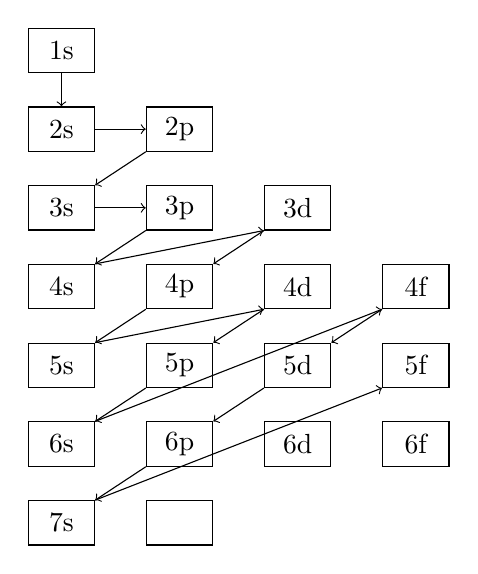
\begin{tikzpicture}
        \draw 
        (1,-0.5) node[draw,minimum width = 2.4em, minimum height = 1.6em] (1s) {1s}
        (1,-1.5) node[draw,minimum width = 2.4em, minimum height = 1.6em] (2s) {2s}
        (1,-2.5) node[draw,minimum width = 2.4em, minimum height = 1.6em] (3s) {3s}
        (1,-3.5) node[draw,minimum width = 2.4em, minimum height = 1.6em] (4s) {4s}
        (1,-4.5) node[draw,minimum width = 2.4em, minimum height = 1.6em] (5s) {5s}
        (1,-5.5) node[draw,minimum width = 2.4em, minimum height = 1.6em] (6s) {6s}
        (1,-6.5) node[draw,minimum width = 2.4em, minimum height = 1.6em] (7s) {7s}
        (2.5,-1.5) node[draw,minimum width = 2.4em, minimum height = 1.6em] (2p) {2p}
        (2.5,-2.5) node[draw,minimum width = 2.4em, minimum height = 1.6em] (3p) {3p}
        (2.5,-3.5) node[draw,minimum width = 2.4em, minimum height = 1.6em] (4p) {4p}
        (2.5,-4.5) node[draw,minimum width = 2.4em, minimum height = 1.6em] (5p) {5p}
        (2.5,-5.5) node[draw,minimum width = 2.4em, minimum height = 1.6em] (6p) {6p}
        (2.5,-6.5) node[draw,minimum width = 2.4em, minimum height = 1.6em] (7p) {\mbox{}}
        (4,-2.5) node[draw,minimum width = 2.4em, minimum height = 1.6em] (3d) {3d}
        (4,-3.5) node[draw,minimum width = 2.4em, minimum height = 1.6em] (4d) {4d}
        (4,-4.5) node[draw,minimum width = 2.4em, minimum height = 1.6em] (5d) {5d}
        (4,-5.5) node[draw,minimum width = 2.4em, minimum height = 1.6em] (6d) {6d}
        (5.5,-3.5) node[draw,minimum width = 2.4em, minimum height = 1.6em] (4f) {4f}
        (5.5,-4.5) node[draw,minimum width = 2.4em, minimum height = 1.6em] (5f) {5f}
        (5.5,-5.5) node[draw,minimum width = 2.4em, minimum height = 1.6em] (6f) {6f}
        ;
        \draw[->] (1s.south) -- (2s.north);
        \draw[->] (2s.east) -- (2p.west);
        \draw[->] (2p.south west) -- (3s.north east);
        \draw[->] (3s.east) -- (3p.west);
        \draw[->] (3p.south west) -- (4s.north east);
        \draw[->] (4s.north east) -- (3d.south west);
        \draw[->] (3d.south west) -- (4p.north east);
        \draw[->] (4p.south west) -- (5s.north east);
        \draw[->] (5s.north east) -- (4d.south west);
        \draw[->] (4d.south west) -- (5p.north east);
        \draw[->] (5p.south west) -- (6s.north east);
        \draw[->] (6s.north east) -- (4f.south west);
        \draw[->] (4f.south west) -- (5d.north east);
        \draw[->] (5d.south west) -- (6p.north east);
        \draw[->] (6p.south west) -- (7s.north east);
        \draw[->] (7s.north east) -- (5f.south west);
        ;
    \end{tikzpicture}
\end{figure}
\begin{ex}
    碱金属内层填满, 故仅有最外层原子对自旋的贡献, 故基态为 \ce{^1S_{1/2}}.
\end{ex}
引入等效电荷$Z^*$后光谱项可表示为
\[ T = \frac{RZ^{*2}}{n^2} \Rightarrow \sqrt{\frac{T}{R}} = \rec{n}\pare{Z-\sigma}. \]
其中$\sigma$谓屏蔽参数. 因此若将$\sqrt{T/R}$对$Z$作图, 可得斜率为$1/n$的直线, 从而确定外层电子的$n$.
\begin{resume}
    \begin{theorem}[Hund规则]
    \begin{cenum}
        \item 对于一个给定的电子组态形成的一组原子态, 当某原子态具有的$S$最大时其所处的能级位置最低.
        \item 对于同一个$S$, $L$最大时能级位置最低.
        \item 对于同科电子, 同一$l$值而$J$不同的能级次序,
        \begin{cenum}
            \item 当同科电子数小于或等于闭壳层占有数一半时具有最小$J$值(即$\abs{L-S}$)的能级处于最低, 谓正常次序.
            \item 当同科电子数大于闭壳层占有数的一半时, 具有最大$J$值(即$L+S$)的能级为最低, 谓倒转次序.
        \end{cenum}
    \end{cenum}
    \end{theorem}
    \begin{theorem}[Land\'e间隔定则]
        在三重态中, 一对相邻的能级之间的间隔与两个$J$值中较大的那个成正比.
    \end{theorem}
\end{resume}
\begin{ex}
    \ce{sp}组态可以给出 \ce{^1P_1}和 \ce{^3P_{2,1,0}}四个状态. 碳, 硅, 锗, 硒, 铅等元素的第一激发态如此. 按照Hund定则, \ce{^1P}态能量高于 \ce{^3P}态, 而 \ce{^3P}相应的三个状态服从正常次序, 其能量差值比为$2:1$.
\end{ex}
\begin{remark}
    轻元素的激发态才适用$J$-$J$耦合, 才适用Hund定则.
\end{remark}
\begin{ex}
    碳族元素的基态最外层有两个 \ce{p}电子, 可以合成 \ce{^1S}, \ce{^1D}, \ce{^3P}, 根据Hund定则, 三个状态中 \ce{^3P}最低. 在 \ce{^3P_2}, \ce{^3P_1}和 \ce{^3P_0}中选择,因为同科电子数小于等于闭壳层占有数的一半, 故$J$值最小的能级最低, 故 \ce{^3P_0}是基态.
\end{ex}
\begin{ex}
    氧原子最外层组成 \ce{p^4}, 可以合成 \ce{^1S}, \ce{^1D}, \ce{^3P}, 根据Hund定则, 同样选取 \ce{^3P}, 但由于同科电子数大于闭壳层占有数的一半, $J$值大的为基态, 即 \ce{^3P_2}.
\end{ex}
Land\'e间隔定则可以解释为自旋磁矩引发的能量差
\begin{align*}
    \Delta E \sim \+v\mu \cdot \+vB \sim \hat S\hat L \cos\expc{\+vL,\+vS} &= \hat S \hat L \frac{\hat J^2 - \hat L^2 - \hat S^2}{2\hat L \hat S}\\ &\sim J\pare{J+1} - L\pare{L+1} - S\pare{S+1}.
\end{align*}
故$J+1$和$J$的能级间距正比于$2\pare{J+1}$.

% subsubsection 壳层的次序 (end)

\subsubsection{电离能变化的解释} % (fold)
\label{ssub:电离能变化的解释}

\begin{cenum}
    \item \ce{He}的两个电子处于同一壳层, 相互静电屏蔽作用小, 故受到吸引力大, 故结合能大.
    \item 对于\ce{Li}, 最外层电子受到的吸引大致等效为$+e$电荷, 故结合能较小.
    \item \ce{Be}由于最外层电子处于同一壳层, 屏蔽效应小于核子电荷增加量, 故结合能变大.
    \item \ce{B}由于壳层升高, 故结合能变小. 其后结合能再度增大. 
    \item 到 \ce{O}出现反常, 因为相互平行的电子数目减少了, 电子重叠部分增加, 故结合能降低.
\end{cenum}

% subsubsection 电离能变化的解释 (end)

% subsection 元素周期表 (end)

\subsection{波函数的对称性与Pauli不相容原理} % (fold)
\label{sub:波函数的对称性与pauli不相容原理}

设两个全同粒子组成一体系有波函数$\psi\pare{1,2}$, 则交换算子$P$成立$P\psi\pare{1,2} = \psi\pare{2,1} = \lambda \psi\pare{1,2}$. 可知$\lambda = \pm 1$. 取正号时谓对称波函数, 反之谓反对称波函数.
\par
若体系的波函数有两种形式,
\[ \psi\+_I_ = \psi_a\pare{1}\psi_b\pare{2},\quad \psi\+_II_ = \psi_b\pare{1}\psi_a\pare{2}, \]
两种形式出现概率等价, 从而总的波函数为
\begin{align*}
    \psi\+_S_\pare{1,2} &= \rec{\sqrt{2}}\brac{\psi_a\pare{1}\psi_b\pare{2} + \psi_b\pare{1}\psi_a\pare{2}}, \\
    \psi\+_A_\pare{1,2} &= \rec{\sqrt{2}}\brac{\psi_a\pare{1}\psi_b\pare{2} - \psi_b\pare{1}\psi_a\pare{2}}.
\end{align*}
分别对应对称与反对称情形. 全同Fermion组成的体系必定有反对称的波函数. 自旋的合成有如下形式:
\begin{align*}
    \psi\+_S,S_ &= \begin{cases}
        \chi_{1,1} = \uparrow\pare{1} \uparrow\pare{2}, \\[1em]
        \chi_{1,0} = \displaystyle \rec{\sqrt{2}}\brac{\uparrow\pare{1} \downarrow\pare{2} + \uparrow\pare{2} \downarrow\pare{1}}, \\[1em]
        \chi_{1,-1} = \downarrow\pare{1} \downarrow\pare{2}.
    \end{cases} \\
    \psi\+_S,A_ &= \chi_{0,0} = \rec{\sqrt{2}}\brac{\uparrow\pare{1} \downarrow\pare{2} - \uparrow\pare{2} \downarrow\pare{1}}.
\end{align*}
由于交换对称性与$z$分量无关, 故$\chi_{1,0}$和$\chi_{0,0}$分别对应$S=1$和$S=0$. 因此结合空间波函数后, 总的波函数可以写为
\[ \psi = \curb{\phi_0\pare{r_1}\phi_{nl}\pare{r_2} - \phi_0\pare{r_2}\phi_{nl}\pare{r_1}} \begin{pmatrix}
    \chi_{1,1} \\
    \chi_{1,0} \\
    \chi_{1,-1}
\end{pmatrix}, \]
或
\[ \psi = \curb{\phi_0\pare{r_1}\phi_{nl}\pare{r_2} + \phi_0\pare{r_2}\phi_{nl}\pare{r_1}} \chi_{0,0}. \]
其中$0$表示基态, $nl$表示某一激发态.
\par
若$S=1$, 则空间波函数具有反对称性, $r_1\neq r_2$, 故两粒子无法靠拢. $S=0$, 则两粒子可以靠拢, 从而经典排斥能变大, 不稳定. 这解释了Hund第一定则.
\par
空间波函数正比于$Y_{l,m}$. 对于二粒子体系$Y_{l,m}\sim \pare{-1}^L$, 从而对于Fermion,
\begin{cenum}
    \item $L$为偶数, 空间波函数$\phi_l$对称从而自旋$\chi$反对称.
    \item $L$为奇数, 空间波函数$\phi_l$反对称从而自旋$\chi$对称.
\end{cenum}
因而对于 \ce{p^2}体系, $L = 2,1,0$, 相应的状态为 \ce{^1D}, \ce{^3P}, \ce{^1S}.

% subsection 波函数的对称性与pauli不相容原理 (end)

\subsection{分子光谱} % (fold)
\label{sub:分子光谱}

电子能级, 振动能级和转动能级的数量级大约为
\[ \Delta E\+_e_ = 1\sim 10\SI{}{\eV},\quad \Delta E\+_vib_ = 10^{-2}\sim 10^{-1}\SI{}{\eV},\quad \Delta E\+_rot_ = 10^{-4}\sim 10^{-2}\SI{}{\eV}.  \]
转动谱在微波/远红外区, 振动谱线在近红外区, 分子的电子能级之间的跃迁在可见光和紫外区.
\par
双原子分子具有轴对称性, 故$z$轴上的角动量守恒, 取$m_l$为相应的量子数, $\lambda = \abs{m_l}$, 则$L_z = \pm m_l \hbar$, $m_l = 0,\pm 1,\pm 2,\cdots$. $\lambda = 0, 1, 2, 3, 4, \cdots$对应的电子态分别用$\sigma$, $\pi$, $\delta$, $\varphi$, $\gamma$, $\cdots$表示.
\par
所有电子的轴向角动量加起来, 得到
\[ \Lambda = \abs{\sum_i \pare{m_l}_i},\quad L = \Lambda \hbar. \]
$\Lambda = 0,1,2,3,4,\cdots$对应的分子态分别用$\Sigma, \Pi, \Delta, \Phi, \Gamma$表示. 总的自旋角动量不受影响, 仍用$M_S$标记, 以$\Sigma$表示, 则$\Sigma$可取$S,S-1,\cdots, -S+1,-S$共$2S+1$个值.
\par
轴向角动量
\[ \Omega = \abs{\Gamma + \Sigma}, \]
可以取$\Lambda + S, \Lambda+S-1,\cdots,\Lambda-S$共$2S+1$个值.
\par
双原子分子的电子态的跃迁满足选择规则
\[ \Delta \Lambda = 0, \pm 1,\quad \Delta S = 0. \]
转动能级为
\[ E\+_rot_ = \frac{\hbar^2}{2I}J\pare{J+1}. \]
选择定则为
\[ \Delta J = \pm 1. \]
\begin{remark}
    只有极性分子才能通过光的吸收或发射发生转动能级间的跃迁. 否则须通过其它机制.
\end{remark}
振动能级为
\[ E\+_vib_ = \pare{n+\half} \hbar\omega,\quad n = 0,1,2,\cdots. \]
选择定则为
\[ \Delta n = \pm 1. \]

% subsection 分子光谱 (end)

% section 多电子原子 (end)

\end{document}
